\newcommand{\assignmentDate}{November 4th, 2019}

% Add title
%Institute
\begin{tabular*}{\hsize}{l@{\extracolsep{\fill}} r}
	\textsc{Technical University of Berlin}		 \hfill&								 	\\
	Faculty II - Mathematics and Natural Sciences\hfill&									\\
	Institute of Mathematics 					 \hfill&									\\
	Dr. D. Peschka, A. Selahi 		 			 \hfill&									\\
\end{tabular*}

% Title
\begin{center}
	\textbf{\Large{\courseName}}\\
	\vspace{7pt}
	\large{Homework \currentAssignment}\\
	\smallskip
	\normalsize{Submitted on \assignmentDate}
\end{center}

% Group table
\begin{center}
	\vspace{-8pt}
	\begin{tabular}{l c r}
		by \textbf{\groupNumber}		    &	 			  &		 								\\
		\hline
		\texttt{Kagan Atci} 			    & \texttt{338131} & \texttt{Physical Engineering, M.Sc.}\\
		\texttt{Navneet Singh }		 	    & \texttt{380443} & \texttt{Scientific Computing, M.Sc.}\\ 
		\texttt{Daniel V. Herrmannsdoerfer} & \texttt{412543} & \texttt{Scientific Computing, M.Sc.}\\ 
		\hline
	\end{tabular}
\end{center}


% EXERCISE 1
% --------------------------------------------------------------------------------------------------------------------
\addExercise{1}{Ex1}
Given is the following boundary problem of an annulus
\begin{equation}
	\begin{cases}
		-\Delta u = 0, &\text{in } \Omega = \{(x,y) \in \mathbb{R}^2 \colon 1 \leq \sqrt{x^2 + y^2} < 2 \} \subset \mathbb{R}^2, \\
		u = g, &\text{on } \partial \Omega,
	\end{cases}
	\label{eq:annulus1}
\end{equation}
with the boundary condition
\begin{equation}
	g(x,y) = 
	\begin{cases}
		x &\text{for } x^2 +y^2 = 2^2\\
		0 &\text{otherwise}
	\end{cases}
\end{equation}
%
% ----------------
\addSubExercise{a}
$(x,y) \in \Omega$ is transformed to polar coordinates $(r, \varphi) \in \Omega_r$ using
\begin{align}
	x &= r \cos{(\varphi)},\\
	y &= r \sin{(\varphi)}
\end{align}
with $r \in (1,2]$ and $\varphi \in (0, 2 \pi]$. Let $v:\Omega_r \to \mathbb{R}$ defined by $v(r,\varphi) = v(x,y)$.
In this case, the partial derivatives $v_x$ and $v_y$ are expressed using chain rule as follows
\begin{align}
	%\frac{}{}
	\label{eq:chainX}
	\frac{\partial v}{\partial x} &= \frac{\partial v}{\partial r} \frac{\partial r}{\partial x} +
									\frac{\partial v}{\partial \varphi} \frac{\partial \varphi}{\partial x}, \text{also denoted as } u_x = u_r r_x + v_\varphi \varphi_x\\
	%
	\label{eq:chainY}
	\frac{\partial v}{\partial x} &= \frac{\partial v}{\partial r} \frac{\partial r}{\partial x} +
									\frac{\partial v}{\partial \varphi} \frac{\partial \varphi}{\partial x}, \text{also denoted as } u_y= u_r r_y + v_\varphi \varphi_y
\end{align}
%
The second partial derivative of $v$ with respect to $x$ is obtained using product rule
\begin{equation}
	v_{xx} = u_r r_{xx} + (u_r)_x r_x + v_\varphi \varphi_{xx} + (v_\varphi)_x \varphi_x
	\label{eq:uXX}
\end{equation}
%
By applying the chain rule from \EQ{chainX} and \EQ{chainY} into  \EQ{uXX}, $v_{xx}$ is written in the following form
%
\begin{equation}
	v_{xx} = u_r r_{xx} + v_{rr} r_{x}^2 + 2 v_{r\varphi} r_x \varphi_x + v_\varphi \varphi_{xx} + v_{\varphi \varphi} \varphi_x^2
	\label{eq:uXX_chain}
\end{equation}
%
where a similar expression is obtained for y
\begin{equation}
	v_{yy} = u_r r_{yy} + v_{rr} r_{y}^2 + 2 v_{r\varphi} r_y \varphi_y + v_\varphi \varphi_{yy} + v_{\varphi \varphi} \varphi_y^2
	\label{eq:uYY_chain}
\end{equation}
%
The laplace equation $\Delta v = v_{xx} + v_{yy}$ can be written in a proper semi-polar coordinate form by adding \EQ{uXX_chain} and \EQ{uYY_chain} and collecting the like terms
\begin{align}
	\nonumber
	\Delta v &= v_{xx} + v_{yy}\\
	\label{eq:laplaceExpanded}
			 &= u_r(r_{xx} + r_{yy}) + v_{rr} (r_x^2 + r_y^2) + 2 v_{r\varphi} (r_x \varphi_{x} + r_y \varphi_y) + v_\varphi (\varphi_{xx} + \varphi_{yy}) + v_{\varphi\varphi} (\varphi_x^2 + \varphi_y^2)
\end{align}
%
Now, expressions in parentheses are to be elaborated in the partial derivations with respect to polar coordinates.
For this purpose, the relationship $x^2 + y^2 = r^2$ is differentiated with respect to x and y.
Accordingly, the partial differentiation of $r$ terms with respect Cartesian terms up to second order are obtained as
\begin{align}
	\label{eq:r_x}	
	r_x    &= \frac{x}{r},\\
	r_{xx} &= \frac{y^2}{r^3},\\
	r_{y}  &= \frac{y}{r},\\
	r_{yy} &= \frac{x^2}{r^3}\text{.}
\end{align}
%
Similarly, the partial differentiation of $\varphi$ terms with respect to x and y are obtained as
\begin{align}
	\varphi_x    &= -\frac{y}{r^2},\\
	\varphi_{xx} &= \frac{2xy}{r^4},\\
	\varphi_{y}  &= \frac{x}{r^2},\\
	\label{eq:phi_yy}
	\varphi_{yy} &= -\frac{2xy}{r^4}\text{.}
\end{align}
%
Employing the Equations \ref{eq:r_x} to \ref{eq:phi_yy} in \EQ{laplaceExpanded} gives
\begin{align*}
	\Delta v &= u_r\left(\frac{y^2}{r^3} + \frac{x^2}{r^3}\right) + v_{rr} \left(\left(\frac{x}{r} \right)^2+ \left(\frac{y}{r} \right)^2\right) + 2 v_{r\varphi} \left(\frac{-xy}{r^3}+\frac{yx}{r^3}\right) + \hdots\\
			 &v_\varphi \left(\frac{2xy}{r^4} - \frac{2xy}{r^4}\right) + v_{\varphi\varphi} \left(\left(-\frac{x^2}{r^3}\right) ^2 + \left(\frac{x^2}{r^3}\right)^2 \right)\\
			 &= \frac{1}{r} u_r + v_{rr} + 0 + 0 + \frac{1}{r^2} v_{\varphi\varphi}.
\end{align*}
Thus, for any $v$ satisfying the Laplace equation $-\Delta v = 0$, $v$ satisfies in polar coordinates the equation
\begin{equation}
	\label{eq:laplacePolar}
	-\left(v_{rr} + \frac{1}{r} v_r + \frac{1}{r^2} v_{\varphi\varphi}\right)=0
\end{equation}
%
% ----------------
\addSubExercise{b}
For any $v$ defined in a), the domain $\Omega_v$ is defined as
\begin{equation}
	\Omega_v = \{(r,\varphi) \in \mathbb{R}^2 \colon r \in (1,2), \varphi \in (0, 2\pi]\}
\end{equation}
with the boundary condition 
\begin{equation}
	\label{eq:boundaryPolar}
	h(r, \varphi) =
	\begin{cases}
		2\cos{(\varphi)} &\text{ for } r = 2,  \varphi \in (0, 2\pi] \\
		0 &\text{otherwise}
	\end{cases}
\end{equation}
%
% ----------------
\addSubExercise{c}
\newcommand{\constFac}{\lambda}
Assuming that $v(r,\varphi) = R(r)\Phi(\varphi) \text{, } \forall r \in (0,1] \text{, } \forall \varphi \in (0,2\pi]$.
If $v(r,\varphi)$ satisfies \EQ{laplacePolar}, then this equation can be expressed in the following form
\begin{equation}
	\label{eq:laplaceSep}
	-\left(R_{rr} \Phi + \frac{1}{r} R_r \Phi + \frac{R}{r^2} \Phi_{\varphi\varphi}\right) = 0
	\text{.}
\end{equation}
Placing the functions depended of $r$ and $\varphi$ in separate terms, \EQ{laplaceSep} is written as
\begin{equation}
	\label{eq:laplaceSep2}
	\frac{r^2 R_{rr} + r R_r}{R} = -\frac{\Phi_{\varphi\varphi}}{\Phi} = -\constFac
\end{equation}
where $\constFac$ represent a constant real factor.
\EQ{laplaceSep2} enables $v(r,\varphi)$ to be considered as two different ODE's, as both $R$ and $\Phi$ terms are equated with $\constFac$ separately
%
\begin{align}
	\label{eq:odePhi}
	\frac{\Phi_{\varphi\varphi}}{\Phi} &= \constFac \iff    \Phi_{\varphi\varphi} = \Phi \constFac \\ 
	\label{eq:odeR}
	\frac{r^2 R_{rr} + r R_r}{R} &= \constFac      \iff   \left(r^2 R_{rr} + r R_r \right) = -R \constFac
	\text{.}
\end{align}
%
% ----------------
\addSubExercise{d}
The solution of $v(r,\varphi)$ consists of the superposition of \EQ{odePhi} and \EQ{odeR} solutions, which are studied in three different cases for $\lambda$:
\begin{itemize}
	\item {\boldmath$\lambda = 0$}: \\
		In this case, possible solutions are given by\\
		\begin{align}
			\Phi(\varphi)&= a \varphi + b\\
			R(r)         &= c \ln{r} + d
			\text{.}
		\end{align}
		Since $\Phi$ has to be a periodic equation, $a = 0$, and $c = 0$, as the solution has to remain finite, as $r$ goes to 0.
		With the applied conditions, the ansatz gives
		\begin{equation}
			\label{eq:vLambda1}
			v(r, \varphi) = b d = g = const.
		\end{equation}
%
	\item {\boldmath$\lambda < 0$}: \\
		Let $\lambda = -k^2$.
		Possible solutions for $R$ and $\Phi$ are given by
		\begin{align}
		\label{eq:phiLambda2}
			\Phi(\varphi)&= a_k \cosh{(k\varphi)} + b_k \sinh{(k\varphi)}\\
			R(r)         &= c_k r^{-k} + d_k r^{k}
		\end{align}
		$v(r,\varphi)$ holds no solutions for this case, because \EQ{phiLambda2} implies a periodic function in neither terms, thus remains zero for $\Phi$.
%
	\item {\boldmath$\lambda > 0$}: \\
		Let $\lambda = k^2$.
		Possible solutions are given by
		\begin{align}
		\label{eq:phiLambda3}
			\Phi(\varphi)&= a_k \cos{(k\varphi)} + b_k \sin{(k\varphi)}\\
			R(r)         &= c_k r^{k} + d_k r^{-k}
		\end{align}
		In this case, $\Phi$ shows a well periodic function with period $2\pi$.
		Furthermore $d_k$ must be $-c_k$, in order to apply the boundary condition on the inner edge of the disc
		\begin{equation}
		\label{eq:vLambda3}
			v(r, \varphi) = (r^k - r^{-k}) \left( A_k \cos{(k \varphi)} + B_k \sin(k \varphi)\right)
		\end{equation}
		where $A_k = a_k c_k$ and $B_k = b_k c_k$.
\end{itemize}
The solution for $v(r, \varphi)$ is expressed as the superposition of \EQ{vLambda1} and \EQ{vLambda3}
\begin{equation}
	v(r, \varphi) = g + \sum_{k=1}^{} (r^k - r^{-k}) \left( A_k \cos{(k \varphi)} + B_k \sin(k \varphi)\right)
\end{equation}
for $A_k$ and $B_k \in \mathbb{R}$ are obtained by the Fourier expansion.
\par
The solution of $v(r, \varphi)$ is to be investigated on the outer boundary with $r = 2$.
So gives
\begin{equation}
	\label{eq:vBoundary}
	v(2, \varphi) = g + \sum_{k=1}^{} (2^k - 2^{-k}) \left( A_k \cos{(k \varphi)} + B_k \sin(k \varphi)\right) = 2 \cos{(\varphi)}
\end{equation}
As \EQ{vBoundary} implies, the boundary condition is already given in the Fourier-series form, so that the only solution exists for $k = 1$, $A_1 = \frac{4}{3}$, $B_1 = 0$ and $g=0$.
Hence the solution, that satisfies \EQ{laplacePolar} and \EQ{boundaryPolar} in $\Omega_v$ is
\begin{equation}
	\label{eq:vSol}
	v(r, \varphi) = \left(r - \frac{1}{r}\right) \frac{4}{3} \cos{(\varphi)}
	\text{.}
\end{equation}
%
% ----------------
\addSubExercise{e \& f}
The solution code can be found in \texttt{a02e01solution.m} and the plot code in \texttt{a02e01plot.m}.
The surface plot of the \EQ{vSol} solution is illustrated in \FIG{a02e01plot}.
\begin{figure}[H]
\vspace*{\FigUpperVSpace}
\def\MeshFigWidth{220pt}
	\begin{subfigure}{0.5\hsize}
		\centering
		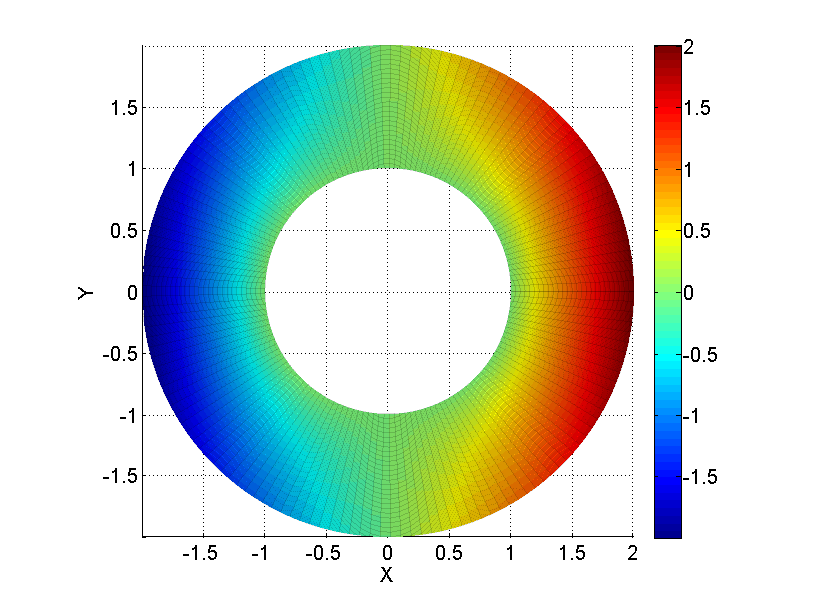
\includegraphics[width=\MeshFigWidth]{a02e01plot_XY.png} 
		\caption{X-Y Plane}
		\label{fig:a02e01plot_XY}
	\end{subfigure}
	\begin{subfigure}{0.5\hsize}
		\centering
		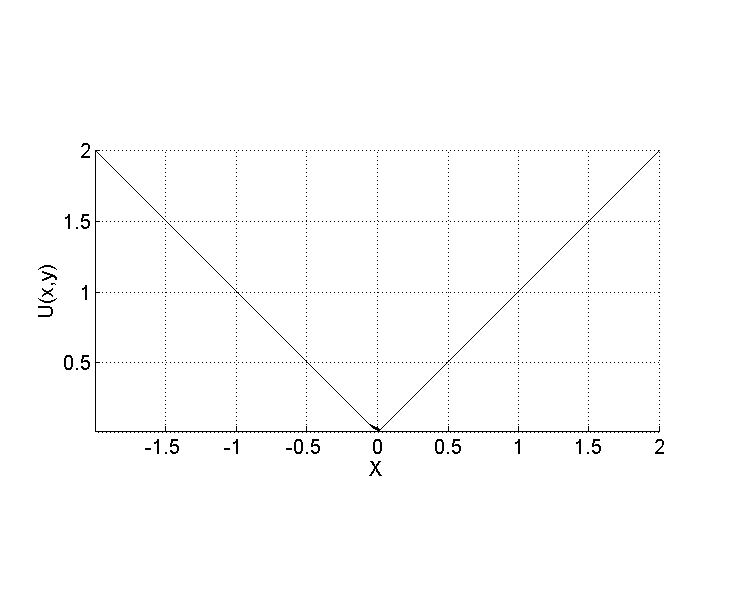
\includegraphics[width=\MeshFigWidth]{a02e01plot_XZ.png} 
		\caption{X-U Plane}
		\label{fig:a02e01plot_XZ}
	\end{subfigure}
	\vfill
	\begin{subfigure}{0.5\hsize}
		\centering
		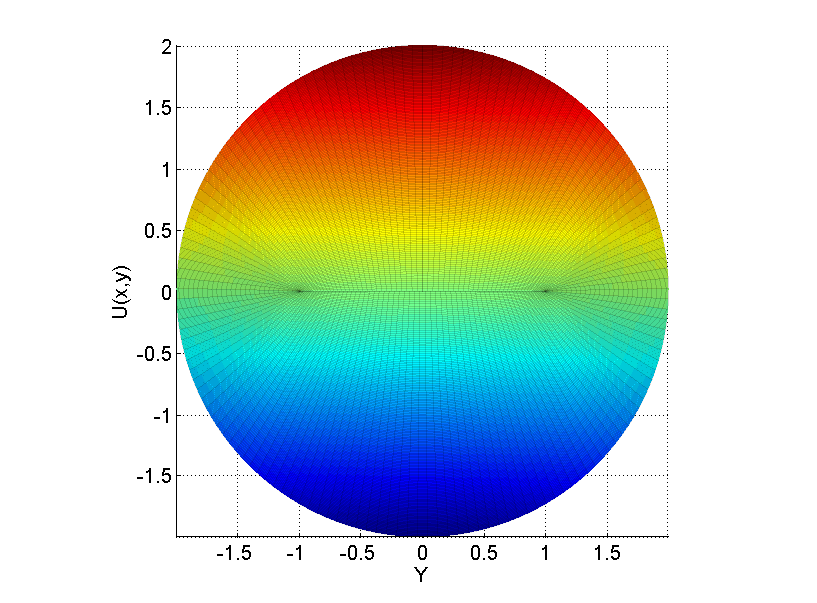
\includegraphics[width=\MeshFigWidth]{a02e01plot_YZ.png} 
		\caption{Y-U Plane}
		\label{fig:a02e01plot_YZ}
	\end{subfigure}
	\begin{subfigure}{0.5\hsize}
		\centering
		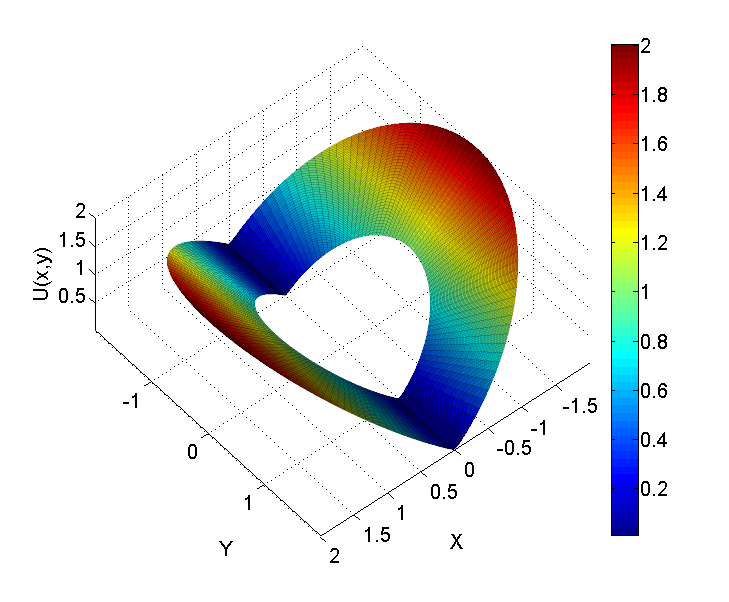
\includegraphics[width=\MeshFigWidth]{a02e01plot_Iso.png} 
		\caption{Isometric View}
		\label{fig:a02e01plot_Iso}
	\end{subfigure}
	\caption{Surface Plot of the Solution}
	\label{fig:a02e01plot}
\end{figure}

% EXERCISE 2
% --------------------------------------------------------------------------------------------------------------------
\addExercise{2}{Ex2}
%
% ----------------
\addSubExercise{a \& b} See the handwritten solutions.

%
% ----------------
\addSubExercise{c \& d}The solution and plot codes can be found in \texttt{NumMat\_Ex2\_2\_Program.py}.
An example of the solution results with respect to input data is illustrated in \FIG{a02e02plot}.
%
\begin{figure}[H]
\vspace*{\FigUpperVSpace}
	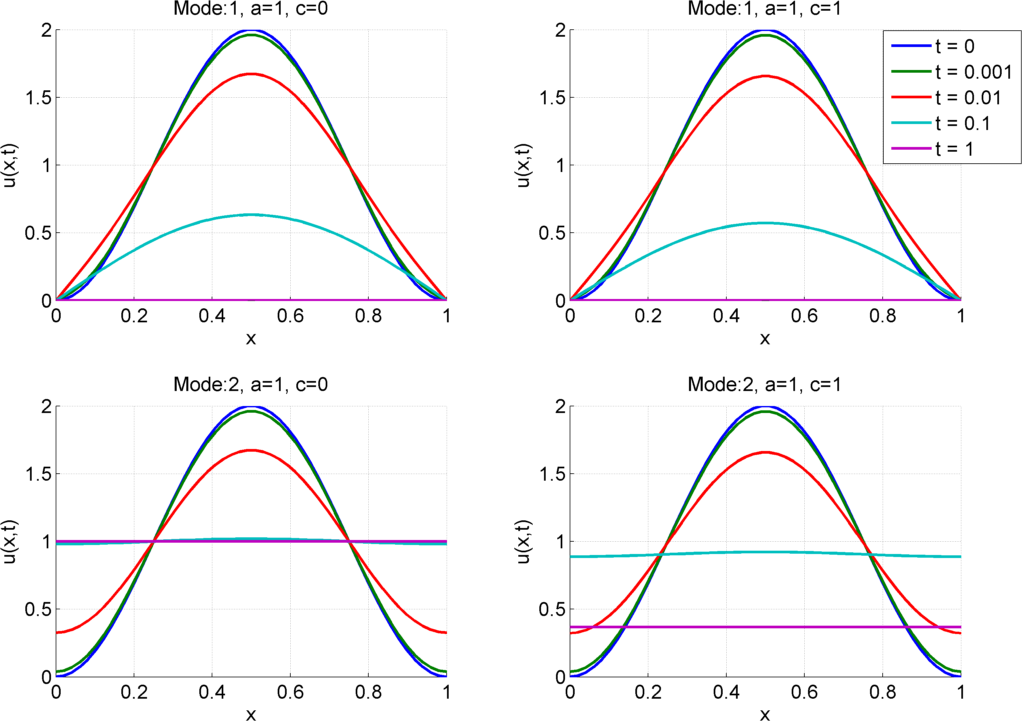
\includegraphics[width=\textwidth]{a02e02plot.png} 
	\caption{Results of the heat-equation with respect to boundary conditions, $a$ and $c$}
	\label{fig:a02e02plot}
\end{figure}

% EXERCISE 3
% --------------------------------------------------------------------------------------------------------------------
\addExercise{3}{Ex3}
Given is $u \colon [0,1] \rightarrow \mathbb{R}$ as a sufficiently smooth function.
% ----------------
\addSubExercise{a}
For $x \in [0,1]$ , following difference quotients are considered:
\begin{align}
	\label{eq:D0}
	D^0u(x) &= \frac{u(x+h) - u(x-h)}{2h}\\
	\label{eq:D+}
	D^+u(x) &= \frac{u(x+h) - u(x)}{h}   \\
	\label{eq:D-}
	D^-u(x) &= \frac{u(x)   - u(x-h)}{h} \\
	\label{eq:D+-}
	D^+D^-u(x) &= \frac{u(x+h) -2u(x)  + u(x-h)}{h^2}
\end{align}
with $ h \in \left(0, \frac{1}{2}\right)$ the given step size.
For the given $x$ interval holds $[x-h < 0, x+h > 1]$.
Hence the x interval of the above mentioned quotients is
\begin{itemize}
	\item $x \in [h, 1-h] \text{ for } D^0$,
	\item $x \in [0, 1-h] \text{ for } D^+$,
	\item $x \in [h,   1] \text{ for } D^-$,
	\item $x \in [h, 1-h] \text{ for } D^+D^-$.\\
\end{itemize}

% ----------------
\addSubExercise{b}
The equality of $D^0(x) = \frac{1}{2}\left(D^+(x) + D^-(x)\right)$ is investigated by employing Equations (\ref{eq:D+}) and (\ref{eq:D-}), and the result must give \EQ{D0}.
\begin{align}
	\nonumber
	\frac{1}{2}(D^+u(x) + D^-u(x)) &= \frac{1}{2}\left(\frac{u(x+h) - u(x)}{h} + \frac{u(x) - u(x-h)}{h} \right)\\
								   \label{eq:D0eq}
								   &= \frac{1}{2}\frac{u(x+h) - u(x-h)}{h}
\end{align}
\EQ{D0eq} confirms the equality for $x\in[0,1]$.
% ----------------
\addSubExercise{c}
Similar to \textbf{b)}, both sides of $D^+D^-u(x) = D^-D^+u(x)$ are investigated separately.
\begin{align}
	\nonumber
	D^+D^-u(x) &= D^+  		  \left[ \frac{u(x) - u(x-h)}{h} \right] \\
	\nonumber
			   &= \frac{1}{2} \left[ D^+ u(x) - D^+ u(x-h) \right] \\
	\nonumber
			   &= \frac{1}{h} \left[ \frac{x(u + h) - u(x)}{h} - \frac{x(u - h + h) - u(x - h)}{h}\right] \\
			   \label{eq:D+-eq}
			   &= \frac{u(x+h) -2u(x)  + u(x-h)}{h^2}
\end{align}
\begin{align}
	\nonumber
	D^-D^+u(x) &= D^-  		  \left[ \frac{u(x+h) - u(x)}{h} \right] \\
	\nonumber
			   &= \frac{1}{2} \left[ D^- u(x+h) - D^- u(x) \right] \\
	\nonumber
			   &= \frac{1}{h} \left[ \frac{x(u + h) - u(x+h-h)}{h} - \frac{x(u) - u(x - h)}{h}\right] \\
			   \label{eq:D-+eq}
			   &= \frac{u(x+h) -2u(x)  + u(x-h)}{h^2}
\end{align}
Equations (\ref{eq:D+-eq}) and (\ref{eq:D-+eq}) confirm the equality for $x\in[0,1]$.

% ----------------
\addSubExercise{d}
Applying Taylor's formula on \EQ{D0} gives
\begin{align}
	\nonumber
	D^0 u(x) &= \frac{1}{2} [\cancel{u(x)} + u^\prime(x)h + \cancel{\frac{1}{2} u^{\prime \prime}(x)h^2} + \frac{1}{6}u^{\prime \prime \prime}(x)h^3 + \cdots \\
			 \nonumber
			 &\quad\;\; \cancel{-u(x)} + u^\prime(x)h \cancel{-\frac{1}{2} u^{\prime \prime}(x)h^2} + \frac{1}{6}u^{\prime \prime \prime}(x)h^3 + \cdots ]		\\
			 &=	u^\prime(x) + h^2\underbrace{\left[\frac{1}{6}u^{\prime \prime \prime}(x) + R \right]}_{R_0}\text{.}
\end{align}
Considering that $R_0 = \frac{1}{6} \left(u^{\prime \prime \prime}(\xi_1) + u^{\prime \prime \prime}(\xi_2) \right)$, it holds
\begin{align}
	\left|R_0\right| \leq \frac{1}{6} \max{\left|u^{\prime \prime \prime}(\xi)\right|}, \text{ for } \xi, \xi_1, \xi_2 \in [x-h, x+h] \text{.}
\end{align}
%
Applying the same procedure on \EQ{D+-} gives
\begin{align}
	\nonumber
	D^{+-} u(x) &= \frac{1}{h^2} [\cancel{u(x)} \cancel{+u^\prime(x)h} + \frac{1}{2} u^{\prime \prime}(x)h^2 \cancel{+ \frac{1}{6}u^{\prime \prime \prime}(x)h^3} + \frac{1}{24} u^{(4)}h^4+ \cdots \\
			 \nonumber
				&\qquad\quad\cancel{u(x)} \cancel{-u^\prime(x)h} - \frac{1}{2} u^{\prime \prime}(x)h^2 \cancel{-\frac{1}{6}u^{\prime \prime \prime}(x)h^3} + \frac{1}{24} u^{(4)}h^4+ \cdots\\
			\nonumber
				&\quad\;\; \cancel{-2u(x)}]\\
				&=	u^\prime(x) + h^2\underbrace{\left[\frac{1}{12}u^{(4)}(x) + R \right]}_{R_1}\text{.}
\end{align}
Considering that $R_1 = \frac{1}{12} \left(u^{(4)}(\xi_1) + u^{(4)}(\xi_2) \right)$, it holds
\begin{align}
	\left|R_1\right| \leq \frac{1}{12} \max{\left|u^{(4)}(\xi)\right|}, \text{ for } \xi, \xi_1, \xi_2 \in [x-h, x+h] \text{.}
\end{align}
$D^-D^0$ is obtained by applying \EQ{D-} on \EQ{D0}
\begin{align}
	\nonumber
	D^-D^0 &= \frac{D^-}{2h}\left(u(x+h) - u(x-h)\right) \\
	\nonumber
		   &= \frac{1}{2h} \left( \frac{u(x+h) - u(x)}{h} - \frac{u(x-h) - u(x-2h)}{h}\right)\\
		   &= \frac{1}{2h} \left( -u(x) + u(x+h) -u(x-h)+u(x-2h)\right)
\end{align}
Hence, the Taylor approximation of $D^-D^0$ is
\begin{align}
	\nonumber
	D^-D^0 = \frac{1}{2h^2}[\;&\cancel{u(x)} + \cancel{u^{\prime}(x) h} \cancel{+ \frac{1}{2} u^{\prime\prime}(x)h^2} + R_1 + \cdots \\
	\nonumber
					          &\cancel{-u(x)} \\
	\nonumber
							  &\cancel{-u(x)} \cancel{+ u^{\prime}(x) h} \cancel{- \frac{1}{2} u^{\prime\prime}(x)h^2} + R_2 + \cdots \\
	\nonumber
							  &\cancel{u(x)} \cancel{- u^{\prime}(x)2h} + \frac{1}{2} u^{\prime\prime}(x)4h^2 - R_3 ]\\
							  \label{eq:D-0}
							  & = \frac{1}{2h^2}\left(2u^{\prime\prime}(x)h^2 +R_1 +R_2 - R_3\right) = u^{\prime\prime} + \mathcal{O}(h)
\end{align}
As \EQ{D-0} implies, this differentiation quotient has a lower order, compared to above mentioned ones.
This shows a lower rate in error decrease and thus less suitable for approximating the second derivative.